
\section{Applications}

\subsection{Exemple d'implémentation d'après un sujet de l'XENS 2015}
On souhaite stocker en mémoire une liste non-ordonnée d'au plus n entiers sans redondance (i.e. ou aucun entier n'apparaît
plusieurs fois). Nous utilisons un tableau 
liste de longueur $n+1$ tel que :
\begin{itemize}
\item liste\verb![!0\verb!]! contient le nombre d'éléments dans le tableau ;
\item liste\verb![!i\verb!]! contient le i\ieme élément de la liste non-ordonnée avec $1\leqslant i \leqslant $\texttt{liste[0]}.
\end{itemize}
Nous disposons d'une fonction \texttt{creerListeVide(n:int)->list} qui permet de créer une liste pouvant contenir $n$ éléments.

\begin{lstlisting}
>>> creerListeVide(3)
        [0,None,None,None]
\end{lstlisting}

Nous disposons d'une fonction \lstinline{estDansListe(liste:list,x)->bool} qui renvoie \lstinline{True} si l'élément $x$ est dans la liste et \lstinline{False} sinon.

La complexité de cette fonction est linéaire en fonction du nombre d'élément maximum que peut contenir la liste. 
Nous disposons aussi d'une fonction \lstinline{ajouteDansListe(liste:list,x)} qui modifie la liste pour ajouter l'élément $x$ s'il n'est pas présent et ne fait rien sinon. La complexité est aussi linéaire du nombre d'élément maximum que peut contenir la liste.

Un plan $P$ est défini par un ensemble de $n$ villes numérotées de $1$ à $n$ et un ensemble de $m$ routes (toutes à double sens)
reliant chacune deux villes. On dira que deux villes $x, y \in  n$ sont voisines lorsqu'elles sont reliées par une route, ce que l'on notera $(x, y)$. On appellera chemin de longueur $k-1$ toute suite de villes $\verb![!v_1, v_2 ... , v_k\verb!]!$. Un plan $P$ est alors un graphe dont les sommets sont les villes et les routes les arêtes.

\textbf{Structure de données. } 

Nous représentons tout plan $P$ à $n$ villes par un tableau plan de $(n+1)$ tableaux où :
\begin{itemize}
\item plan\verb![!0\verb!]! contient un tableau de deux éléments où :
\begin{itemize}
\item plan\verb![!0\verb!]!\verb![!0\verb!]! a pour valeur le nombres $n$ de villes;
\item plan\verb![!0\verb!]!\verb![!1\verb!]! a pour valeur le nombres $m$ de routes.
\end{itemize}
\end{itemize}


\begin{itemize}
\item Pour toute ville $v \in n$, plan\verb![!v\verb!]! contient un tableau à $n$ éléments représentant 
la liste à au plus $(n-1)$ éléments des villes voisines de $v$ dans $P$ dans un ordre arbitraire en utilisant
la structure de liste sans redondance décrite plus haut. Ainsi :
\begin{itemize}
\item plan\verb![!v\verb!]!\verb![!0\verb!]! a pour valeur le nombre de villes voisines de $v$ ;
\item plan\verb![!v\verb!]!\verb![!1\verb!]! , ... ,n\verb![!v\verb!]!\verb![!n\verb![!v\verb!]!\verb![!0\verb!]!\verb!]! sont les indices des villes voisines de $v$.
\end{itemize}
\end{itemize}

\begin{minipage}[c]{.45\linewidth}
\begin{center}
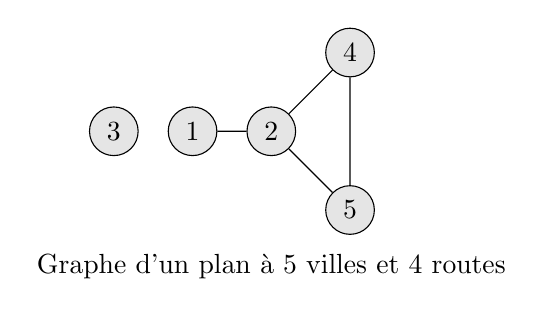
\begin{tikzpicture}[scale=1]
\tikzstyle{sommet}=[circle,draw,fill=gray!20]
\tikzstyle{arete}=[midway,fill=white]
\node[sommet] (S3) at (1,1) {3};
\node[sommet] (S1) at (2,1) {1};
\node[sommet] (S2) at (3,1) {2};
\node[sommet] (S4) at (4,2) {4};
\node[sommet] (S5) at (4,0) {5};
\draw (3,-1) node[above] {Graphe d'un plan à 5 villes et 4 routes} ;
\draw (S1) -- (S2) -- (S4)--(S5)--(S2) ; 
\end{tikzpicture}
\end{center}
\end{minipage}
\hfill
\begin{minipage}[c]{.45\linewidth}
\begin{lstlisting}
plan1= [[5,4] ,
         [1,2,None,None,None],
         [3,4,1,5,None],
         [0,None,None,None,None],
         [2,2,5,None,None],
         [2,4,2,None,None]]
\end{lstlisting}
\end{minipage}
 
\question{ Représenter sous forme de tableaux les deux plans suivants :}
\begin{center}
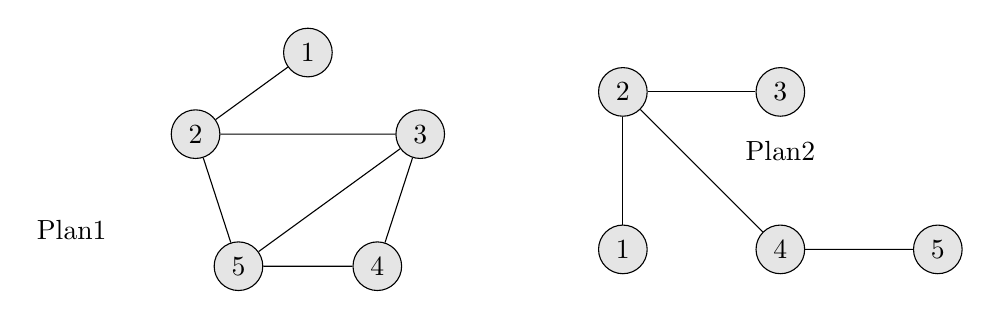
\begin{tikzpicture}[scale=1]
\tikzstyle{sommet}=[circle,draw,fill=gray!20]
\tikzstyle{arete}=[midway,fill=white]
\node[sommet] (A1) at ( 90:1.5) {1};
\node[sommet] (A2) at (162:1.5) {2};
\node[sommet] (A5) at (234:1.5) {5};
\node[sommet] (A4) at (306:1.5) {4};
\node[sommet] (A3) at ( 18:1.5) {3};
\draw (A1)--(A2)--(A3) -- (A4) -- (A5) --(A2);
\draw (A5)--(A3);
\draw (-3,-1) node[above] {Plan1} ;
\node[sommet] (B1) at (4,-1) {1};
\node[sommet] (B2) at (4,1) {2};
\node[sommet] (B3) at (6,1) {3};
\node[sommet] (B4) at (6,-1) {4};
\node[sommet] (B5) at (8,-1) {5};
\draw (6,0) node[above] {Plan2} ;
\draw (B1) -- (B2) -- (B3) ;
\draw (B2) -- (B4) -- (B5) ; 
\end{tikzpicture}
\end{center}


\question{ Écrire une fonction \lstinline{creerPlanSansRoute(n:int)} qui crée, remplit et renvoie le tableau de tableaux correspondant au plan à $n$ villes n'ayant aucune route.}


\question{ Écrire une fonction \lstinline{estVoisine(plan,x,y)} qui renvoie \lstinline{True} si les villes \lstinline{x} et \lstinline{y} sont voisines dans le plan codé par le tableau de tableaux \lstinline{plan} et renvoie \lstinline{False} sinon.}


\question{Écrire une procédure \lstinline{ajouteRoute(plan,x,y)} qui modifie le tableau de tableaux plan pour ajouter une route 
entre les villes \lstinline{x} et \lstinline{y} si elle n'était pas déjà présente et ne fait rien sinon. On prendra garde à bien mettre à jour
toutes les cases concernées dans le tableau de tableaux plan. Y a-t-il un risque de dépassement de la capacité des listes ?}

\question{Écrire une procédure \lstinline{afficheToutesLesRoutes(plan)} qui affiche à l'écran la liste des routes du plan codé par le tableau de tableaux plan
où chaque route n'apparaît qu'une seule fois. Par exemple, pour le graphe codé par le tableau de tableaux de la présentation votre procédure pourra afficher :}
\begin{lstlisting}
`Ce plan contient 4 route(s) : (1-2) (2-4) (2-3) (4-5)`
\end{lstlisting}

\question{Quelle est la complexité de votre procédure ?}
